\documentclass[12pt, a4paper, fleqn, titlepage]{article}

%Packages to use
\usepackage[utf8]{inputenc}
\usepackage{enumerate}
\usepackage{amsmath}
\usepackage{amssymb}
\usepackage{setspace}
\usepackage{array}
\usepackage{ragged2e}
\usepackage{algorithm2e}
\usepackage{graphicx}
\graphicspath{ ./ }
\usepackage[margin=1in]{geometry}

\makeatletter
\renewcommand{\@algocf@capt@plain}{above}% formerly {bottom}
\makeatother


\title{Introduction to Parallel and Distributed Computing: Lab Assignment 2}
\author{Kweku Andoh Yamoa(71712022)}
\date{\today}

%Starting assignment
\doublespacing

\begin{document}
\maketitle
\justify

\section{Introduction}
    The main purpose of this laboratory exercise was to refresh and learn the use of C and then explore,
    learn and apply shared memory programming libraries, i.e., Pthread and OpenMP, for simple
    scientific applications of manipulating very large matrices that are maintained in memory.

\section{Overview}
    To achieve the outcomes of the assignment matrix transposition was the challenge utilised in exploring shared memory libraries. Matrix transposition was done in-place using the basic(brute force) version of the algorithm. After, parallelisation was added to see how shared memory operations optimised memory. Finally, another version of the algorithm was implemented with the use of shared memory libraries. This other algorithm was called Diagonal-Threading.

\section{Basic Algorithm}
    The basic algorithm uses two nested loops to  at index i, and j. For example, the element at A[i][j] will be swapped with the element A[j][i].

    \subsection{Pseudocode}
        \begin{algorithm}[H]
            \CommentSty{Brief: Transposes a given N x N matrix inplace}\\
            \CommentSty{Input:matrix, size(where size = N)}\\
            \CommentSty{Output: Transpose of the given matrix i.e $matrix^T $}\linebreak

            %Main Algorithm
            \For{i $\leftarrow$0 \KwTo size}{
                \For{j $\leftarrow$ i + 1 \KwTo size}{
                    swap(matrix,i,j);
                }
            }

            \begin{flushleft}
                \caption{transposeBasic(matrix, size)}
            \end{flushleft}
        \end{algorithm}    
\section{Pthreads Diagonal} \label{pthreads}

    This section lists and explains diagonal threading using pthreads for matrix transposition.

    \subsection{Overview}
        I used the SPMD(Single Program Multiple Data) design pattern to implement the diagonal-threading algorithm. Two nested loops were used where the outer loop goes through the diagonal elements and the inner loop swaps the row elements at each diagoal
        element to the corresponding column elements. 
        The outer loop iterations are shared among the threads based on the number of threads. To do this, I used formulae to find
        the range of iterations each thread is going to execute given its id. 
        Formulae:
        \[start = (threadId) * \frac{matrix_size}{numThreads};\\
        end = (threadId+1) * \frac{matrix_size}{numThreads}\]

    \subsection{Pseudocode}
        \begin{algorithm}[H]
            \CommentSty{Brief: Transposes a given N x N matrix inplace using pthreads for diagoal threading}\\
            \CommentSty{Input:matrix, size(where size = N)}\\
            \CommentSty{Output: Transpose of the given matrix i.e $matrix^T $}\linebreak
            
            threadId $\leftarrow$ getThreadID() \\
            \CommentSty{\textbackslash\textbackslash compute start and end}\\

            start $\leftarrow (threadId) * \frac{matrix_size}{numThreads}$ \\
            end $\leftarrow (threadId+1) * \frac{matrix_size}{numThreads}$\\

            \For{i $\leftarrow$start \KwTo end}{
                \For{j $\leftarrow$ i + 1 \KwTo size}{
                    swap(matrix,i,j);
                }
            }


            \begin{flushleft}
                \caption{diagoalPthreads(matrix, size)}
            \end{flushleft}
        \end{algorithm}
\section{OpenMP}
    This section talks about naive OpenMP matrix transposition and diagonal threading transposition using OpenMP
    \subsection{Naive OpenMP}
        \subsubsection{Overview}
        The naive OpenMP threading automatically parallelize the code by inserting \#pragma before the for loops. This when compiled ensures that the same basic algorithm is now run in parallel.
        \subsubsection{Pseudocode}
        \begin{algorithm}[H]
            \CommentSty{Brief: Transposes a given N x N matrix inplace using openmp for parallelisation}\\
            \CommentSty{Input:matrix, size(where size = N)}\\
            \CommentSty{Output: Transpose of the given matrix i.e $matrix^T $}\linebreak
                
            nThreads\\
            \#pragma omp parallel\{ \\
                \quad id $\leftarrow$ omp\_get\_num\_threads()\\
                \quad \If{id == 0}{
                    \quad nThreads $\leftarrow$ omp\_get\_num\_thread()\\
                
                    \quad}
                \quad \#pragma omp for nowait \\
                \quad \For{i $\leftarrow$0 \KwTo size}{
                    \quad \For{j $\leftarrow$ i + 1 \KwTo size}{
                        \quad swap(matrix,i,j);
                    }
                }
            \}
            \begin{flushleft}
                \caption{naiveOMPTranspose(matrix, size)
                }
            \end{flushleft}
        \end{algorithm}
    \subsection{Diagonal Threading OpenMP}
        This section gives an overview of diagonal threading using openmp.
        \subsubsection{Overview}
            Diagonal threading using OpenMP is similar to the approach explained for Pthreads Diagonal(See Section \ref{pthreads}). The only distinct difference is for the omp implementation, the loops are parallelised using the \# pragma omp for call.
        \subsubsection{Pseudocode}
            \begin{algorithm}[H]
                \CommentSty{Brief: Transposes a given N x N matrix inplace using openmp for diagoal threading}\\
                \CommentSty{Input:matrix, size(where size = N)}\\
                \CommentSty{Output: Transpose of the given matrix i.e $matrix^T $}\linebreak

                 nThreads\\
                 omp\_set\_dynamic(0) \quad \CommentSty{\textbackslash\textbackslash Explicitly disable dynamic teams} \\
                 omp\_set\_num\_threads(4) \quad \CommentSty{\textbackslash\textbackslash Use 4 threads for all consecutive parallel regions}\\
            \#pragma omp parallel\{ \\
                \quad id $\leftarrow$ omp\_get\_num\_threads()\\
                
                \quad nThreads $\leftarrow$ omp\_get\_num\_thread()\\
                
                
                \quad \CommentSty{\textbackslash\textbackslash compute start and end}\\

                \quad start $\leftarrow (id) * \frac{matrix_size}{nThreads}$ \\
                \quad end $\leftarrow (id+1) * \frac{matrix_size}{nThreads}$\\
                \quad \For{i $\leftarrow$start \KwTo end}{
                    \quad \For{j $\leftarrow$ i + 1 \KwTo size}{
                        \quad swap(matrix,i,j);
                    }
                }
            \}
                
                \begin{flushleft}
                    \caption{diagonalOMPTranspose(matrix, size)
                    }
                \end{flushleft}
            \end{algorithm}
        
\section{Comparative Table of  Performance}
    The table below shows the performance of the various algorithms as implemented in the C programming language.
    \begin{flushleft}
        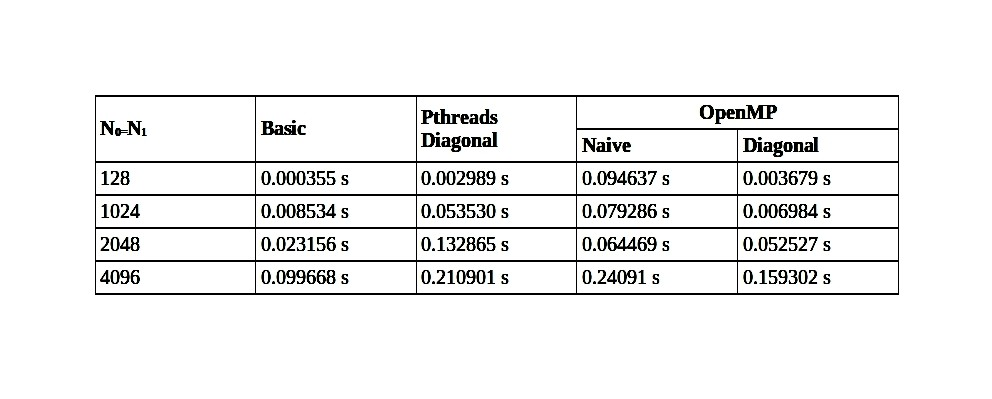
\includegraphics[width= 18cm,height = 10cm, keepaspectratio,scale=0.5]{performance-table}
    \end{flushleft}
\section{Comments on Running Code}
    To run the code successfully for all the sizes of N, make sure that variable \emph{matrix\_size} is changed dynamically to the defined sizes N,N1,N2 and N3.
\end{document}